\input{./econtexRoot.texinput}
\documentclass[\econtexRoot/Chp1proposal]{subfiles}
\onlyinsubfile{\externaldocument{\econtexRoot/Chp1proposal}} % Get xrefs -- esp to apndx -- from main file; only works if main file has already been compiled

\begin{document}

\hypertarget{resultslc}{}
\section{Results for the life cycle model}\notinsubfile{\label{sec:resultslc}}
%\setcounter{page}{0}\pagenumbering{arabic}

\par The additional parameters necessary to calibrate the life cycle version of the model are given in table \ref{tab:calib2}.

\hypertarget{calibLC}{}
\begin{table}[ht]
  \centering
  \resizebox{0.6\textwidth}{!}{
    \begin{tabular}{ccc}
        \toprule
        Description & Parameter & Value  \\
        \midrule
        Population growth rate & $N$ & 0.0025  \\
        Technological growth rate & $\Gamma$ & 0.0037  \\
        Rate of high school dropouts & $\theta_D $ & 0.11  \\
        Rate of high school graduates & $\theta_{HS} $ & 0.55  \\
        Rate of college graduates & $\theta_C $ & 0.34  \\
        Labor income tax rate & $\tau$ & 0.0942  \\
        \bottomrule
    \end{tabular}}
    \caption{Parameter values (annual frequency) for the lifecycle model.}
    \label{tab:calib2}
\end{table}

\unskip

\par The estimation procedure finds this optimal value to be $\Rfree = 1.0078$ for the R-point model in this setting. The estimation procedure for the R-dist model in the life cycle setting finds optimal values of $\Rfree = 1.0005$ and $\nabla = 0.01836$. Consider the improved performance of the estimation in matching the 2004 SCF wealth data, which is compared in figure \ref{fig:LCUnif}.

 \hypertarget{LCUnif}{}
 \begin{figure}[H]
   \centering
   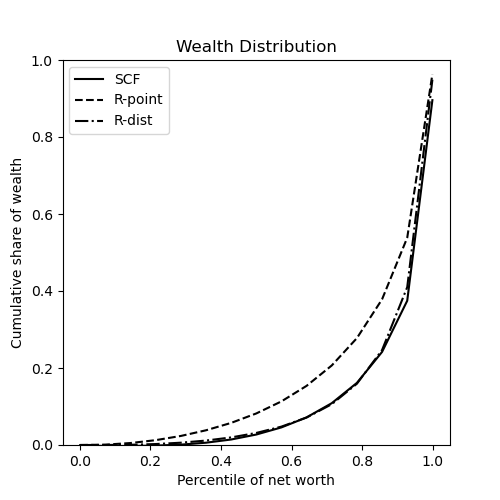
\includegraphics[width=0.7\textwidth]{./Figures/LCUnif.png}
   \caption{Life cycle lorenz curve v.s. data}
    \label{fig:LCUnif}
  \end{figure}\unskip



\onlyinsubfile{% Allows two (optional) supplements to hard-wired \texname.bib bibfile:
% system.bib is a default bibfile that supplies anything missing elsewhere
% Add-Refs.bib is an override bibfile that supplants anything in \texfile.bib or system.bib
\provideboolean{AddRefsExists}
\provideboolean{systemExists}
\provideboolean{BothExist}
\provideboolean{NeitherExists}
\setboolean{BothExist}{true}
\setboolean{NeitherExists}{true}

\IfFileExists{\econtexRoot/Add-Refs.bib}{
  % then
  \typeout{References in Add-Refs.bib will take precedence over those elsewhere}
  \setboolean{AddRefsExists}{true}
  \setboolean{NeitherExists}{false} % Default is true
}{
  % else
  \setboolean{AddRefsExists}{false} % No added refs exist so defaults will be used
  \setboolean{BothExist}{false}     % Default is that Add-Refs and system.bib both exist
}

% Deal with case where system.bib is found by kpsewhich
\IfFileExists{/usr/local/texlive/texmf-local/bibtex/bib/system.bib}{
  % then
  \typeout{References in system.bib will be used for items not found elsewhere}
  \setboolean{systemExists}{true}
  \setboolean{NeitherExists}{false}
}{
  % else
  \typeout{Found no system database file}
  \setboolean{systemExists}{false}
  \setboolean{BothExist}{false}
}

\ifthenelse{\boolean{showPageHead}}{ %then
  \clearpairofpagestyles % No header for references pages
  }{} % No head has been set to clear

\ifthenelse{\boolean{BothExist}}{
  % then use both
  \typeout{bibliography{\econtexRoot/Add-Refs,\econtexRoot/\texname,system}}
  \bibliography{\econtexRoot/Add-Refs,\econtexRoot/\texname,system}
  % else both do not exist
}{ % maybe neither does?
  \ifthenelse{\boolean{NeitherExists}}{
    \typeout{bibliography{\texname}}
    \bibliography{\texname}}{
    % no -- at least one exists
    \ifthenelse{\boolean{AddRefsExists}}{
      \typeout{bibliography{\econtexRoot/Add-Refs,\econtexRoot/\texname}}
      \bibliography{\econtexRoot/Add-Refs,\econtexRoot/\texname}}{
      \typeout{bibliography{\econtexRoot/\texname,system}}
      \bibliography{        \econtexRoot/\texname,system}}
  } % end of picking the one that exists
} % end of testing whether neither exists
}

\ifthenelse{\boolean{Web}}{}{
  \onlyinsubfile{\captionsetup[figure]{list=no}}
  \onlyinsubfile{\captionsetup[table]{list=no}}
}

\end{document} \endinput
